\documentclass{article}

\usepackage[T1]{fontenc}
\usepackage[polish]{babel}
\usepackage[utf8]{inputenc}
\usepackage{graphicx}
\usepackage{xcolor}

\begin{document}
\noindent\makebox[\textwidth]{
\includegraphics[width=\paperwidth]{resources/titlepage.png}}

\raggedleft{\sffamily
    {\Huge\bf\textcolor[HTML]{6495ED}{Szkoła Tańca}}\\\vspace{2em}
    {\Large
        Dokumentacja projektowa PZSP2\\\vspace{1em}
        Wersja 1\\\vspace{1em}
        \today\\\vspace{1em}
        Semestr 25Z%
    }

    \vspace{5em}
    {\large
        Zespół nr 2 w składzie:\\\vspace{0.5em}
        {\rmfamily
        Gavrylenko Ihor\\
        Kukiełka Wojciech\\
        Rybachok Andrii\\
        Yedzeika Sofiya%
        }%
    }%
}

\vspace{3em}
\raggedright{\large
    Mentor zespołu: dr inż. Marcin Szlenk\\
    Właściciel tematu: dr inż. Żółtowska Izabela
}

\newpage

\tableofcontents

\section{Wprowadzenie}
\subsection{Cel projektu}
Celem jest stworzenie aplikacji wspomagającej właścicielkę Szkoły Tip~Tap
w~zarządzaniu ofertą oraz w realizacji bieżących zadań organizacyjnych.
Konkretnie, system ma za zadanie wspomóc właścicielkę i instruktorów
przy realizacji lekcji stepowania, a uczniom ma uprościć formalności
związane z~uczęszczaniem na te zajęcia.

Załączony został dokument \textsc{szkoła tańca.docx,}
zawierający wymagania właścicielki.

\subsection{Wstępna wizja projektu}
Sercem systemu będzie aplikacja webowa, która będzie komunikować się z~serwerem aplikacyjnym.
Będzie stworzona baza danych.
W aplikacji będą trzy rodzaje użytkowników: uczniowie, instruktorzy i administrator.
Podczas projektowania będzie kładziony nacisk na łatwość obsługi, automatyzację czynności
i bezpieczeństwo danych osobowych.

\section{Metodologia wytwarzania}

Nasz zespół składa się z 4-ech osób. Mamy mentora, z którym będziemy się
spotykać co około 3 tygodnie. Stosujemy podejście zwinne, więc jego rolą nie jest
zarządzanie, lecz wsparcie merytoryczne.

Sami w swojej strukturze też nie mamy przewodniczącego, który przydziela zadania,
aczkolwiek mamy lidera -- Ihora, który jest z nas najbardziej doświadczony.
Każdy członek zespołu jest zmotywowany powodzeniem projektu i sam podejmuje się
zadań, biorąc pod uwagę swoje siły i~kompetencje.

\subsubsection*{Schemat pracy}
Głównym spoiwem zespołu są cotygodniowe spotkania, na których przedstawiamy
postępy, dzielimy się spostrzeżeniami i określamy dalsze kierunki działania.
Poza spotkaniami pracujemy, samodzielnie lub w parach.

\paragraph{Role}
Kluczowe jest, aby co najmniej dwie osoby potrafiły zrobić dowolną czynność
deweloperską bądź administracyjną. Chcąc zaspokoić to oczekiwanie,
zadbaliśmy o to, żeby równomiernie przypisać ludzi do odpowiedzialności.
Dokładnie, projekt ma 3 komponenty -- bazę danych, front-end i back-end.
Każdym komponentem zajmują się co najmniej dwie osoby.

\paragraph{Narzędzia}
Podstawą jest narzędzie kontroli wersji -- \textit{git}. Oprócz tego potrzebne jest
miejsce do określania zadań. Obie te funkcje ma platforma \textit{gitlab}.

Mówiąc bardziej technicznie, jednostka pracy (zadanie, issue) będzie odnotowywane
w \textit{gitlabie}, wolontariusz przypisze to zadania do siebie do wykonania,
utworzy niezależną gałąź z kodem, zaimplementuje, co trzeba, a~następnie oznaczy
gałąź, jako gotową do wdrożenia do oficjalnej wersji kodu. Przed wdrożeniem,
gałąź będzie musiała przejść, w pierwszej kolejności -- testy automatyczne,
a następnie recenzję innego członka zespołu.


\section{Analiza wymagań}

\subsection{Wymagania użytkownika i biznesowe}
\newcommand{\wymaganie}[2]{
    \textbf{\textsc{#1}}\hspace{1em}#2\\\vspace{0.5em}
}
\subsubsection*{Wymagania biznesowe}
\wymaganie{B1}{System \textbf{musi} odciążyć właścicielkę w rejestracji uczniów, ich rozliczaniu oraz w kontakcie z nimi.}
\wymaganie{B2}{Aplikacja \textbf{musi} pozwolić rejestrować obecności uczniów.}
\wymaganie{B3}{Aplikacja \textbf{musi} pozwolić uczniom zarejestrować się na zajęcia.}
\wymaganie{B4}{Aplikacja \textbf{musi} wyposażyć uczniów w informacje dotyczące ich uczestnictwa w zajęciach,
    aby, w szczególności, dotrzymywanie terminów płatności było dla nich łatwiejsze.}
\wymaganie{B5}{Aplikacja \textbf{musi} pozwolić właścicielce zmieniać ceny karnetów
    oraz wprowadzać inne zmiany istotne z punktu widzenia systemu.}
\wymaganie{B6}{Aplikacja \textbf{powinna} pozwalać na tworzenie raportów dotyczących sprzedaży karnetów.}

\vspace{-0.5em}
\subsubsection*{Wymagania użytkownika}
Powyższe wymagania pociągają za sobą poniższe wymagania użytkownika.

\vspace{1em}
\wymaganie{U1}{Uczeń \textbf{musi} móc się zarejestrować i zalogować adresem e-mail.}
\wymaganie{U2}{Rejestracja \textbf{powinna} wymagać zatwierdzenia automatycznego e-maila.}
\wymaganie{U3}{Pomyślne zarejestrowanie się \textbf{musi} być jasno zakomunikowane,
    w~szczególności komunikat o tym zdarzeniu powinien być trudny do przeoczenia.}
\wymaganie{U4}{Uczeń \textbf{musi} móc zapisać się na zajęcia.}
\wymaganie{U5}{Uczeń \textbf{powinien} móc wpisać się na listę rezerwową.}
\wymaganie{U6}{Uczeń \textbf{musi} widzieć status swoich płatności}
\wymaganie{U7}{Uczeń \textbf{musi} widzieć ile przysługuje mu odrobień.}
\wymaganie{U8}{Dwaj uczniowie \textbf{muszą} móc mieć ten sam e-mail.}
\wymaganie{U9}{Uczeń \textbf{musi} móc usunąć swoje konto, prosząc o usunięcie jego danych z~systemu.}

\vspace{1em}
\wymaganie{I1}{Instruktor \textbf{musi} móc odnotować obecność ucznia na zajęciach.}
\wymaganie{I2}{Instruktor \textbf{musi} móc odnotować obecność ucznia odrabiającego zajęcia.}
\wymaganie{I3}{Instruktor \textbf{musi} móc skorygować obecność ucznia do 7 dni po zajęciach.}
\wymaganie{I4}{Instruktor \textbf{musi} mieć dostęp \textbf{tylko} do niezbędnych danych,
    w~szczególności \textbf{nie może} mieć dostępu do e-maili.}

\vspace{1em}
\textit{Uwaga: właścicielka jest administratorem.}\\\vspace{0.5em}
\wymaganie{A1}{Administrator \textbf{musi} móc modyfikować grafik zajęć.}
\wymaganie{A2}{Administrator \textbf{musi} móc dodawać konta instruktorów.}
\wymaganie{A3}{Administrator \textbf{powinien} móc modyfikować dane uczniów.}
\wymaganie{A4}{Administrator \textbf{powinien} móc wygenerować podsumowanie płatności z~karnetów za dany okres.}
\wymaganie{A5}{Administrator \textbf{musi} móc odnotować płatność ucznia.}
\wymaganie{A6}{Administrator \textbf{powinien} móc zapisać płatność \textit{w przód,} np. uczeń opłaca za dwa miesiące.}
\wymaganie{A7}{Administrator \textbf{musi} mieć dostęp do danych ucznia, który ma nieuregulowane płatności,
    nawet jeśli usunął konto.}
\wymaganie{A8}{Administrator \textbf{powinien} móc wysłać maila do całej grupy zajęciowej.}

\subsection{Wymagania funkcjonalne i niefunkcjonalne}
Wszystkie powyższe wymagania oprócz \textbf{\textsc{U3}} są przeważnie funkcjonalne,
lecz oczywiste jest, że aby je zrealizować, trzeba spełnić kilka wymagań niefunkcjonalnych.

\vspace{1em}
\wymaganie{N1}{Interfejs \textbf{musi} być prosty, czytelny oraz mieć komunikaty o~sukcesach/błędach.}
\wymaganie{N2}{Systemu \textbf{musi} być dostępny całodobowo z poziomu przeglądarki.}
\wymaganie{N3}{Interfejs \textbf{musi} być równie dobry na urządzeniach mobilnych.}
\wymaganie{N4}{Dane osobowe \textbf{muszą} być przechowywane bezpiecznie z poszanowaniem RODO.}
\wymaganie{N5}{System \textbf{musi} być utrzymywalny.}

\subsubsection*{Mapowania wymagań}
\newcommand{\x}{\rule[-0.25em]{1em}{1em}}
\resizebox{\textwidth}{!}{%
\begin{tabular}{*{22}{c|}}
    \cline{2-22}
    {}                       & U1 & U2 & U3 & U4 & U5 & U6 & U7 & U8 & U9 & I1 & I2 & I3 & I4 & A1 & A2 & A3 & A4 & A5 & A6 & A7 & A8 \\\hline
    \multicolumn{1}{|c|}{B1} &    &    &    &    &    &    &    &    &    &    &    &    &    &    &    &    &    & \x & \x & \x & \x \\\hline
    \multicolumn{1}{|c|}{B2} &    &    &    &    &    &    &    &    &    & \x & \x & \x & \x &    &    &    &    &    &    &    &    \\\hline
    \multicolumn{1}{|c|}{B3} &    &    &    & \x & \x &    &    &    & \x &    &    &    &    &    &    &    &    &    &    &    &    \\\hline
    \multicolumn{1}{|c|}{B4} & \x & \x & \x &    &    & \x & \x & \x &    &    &    &    &    &    &    &    &    &    &    &    &    \\\hline
    \multicolumn{1}{|c|}{B5} &    &    &    &    &    &    &    &    &    &    &    &    &    & \x & \x & \x &    &    &    &    &    \\\hline
    \multicolumn{1}{|c|}{B6} &    &    &    &    &    &    &    &    &    &    &    &    &    &    &    &    & \x &    &    &    &    \\\hline
\end{tabular}}

\subsection{Przypadki użycia}
\newcommand{\przypadek}[2]{\subsubsection*{#1\hspace{1em}#2}}
\przypadek{PB1}{Rejestracja ucznia}
\begin{enumerate}
    \item Uczeń wypełnia formularz rejestracyjny.
    \item System wysyła e-mail weryfikacyjny.
    \item Uczeń potwierdza adres e-mail.
    \item System aktywuje konto i potwierdza rejestrację.
\end{enumerate}

\przypadek{PB2}{Zapisanie się na zajęcia}
\begin{enumerate}
    \item Uczeń przegląda dostępne terminy zajęć.
    \item Uczeń wybiera termin.
    \item Uczeń potwierdza zapis.
    \item System sprawdza, czy miejsce jest wolne.
    \begin{enumerate}
        \item Jeśli tak, zapis jest rejestrowany w systemie.
        \item Jeśli nie, uczeń jest powiadamiany o błędzie.
    \end{enumerate}
\end{enumerate}

\przypadek{PB3}{Przegląd informacji o koncie ucznia}
\begin{enumerate}
    \item Uczeń klika na przycisk „Moje Konto”.
    \item Wyświetla się ogólna informacja o koncie: imię, nazwisko itp.
    \item Menu zawiera następujące zakładki:
    \begin{enumerate}
        \item Lista zajęć, na które uczeń jest zapisany
        \item Dziennik obecności, gdzie uczeń może widzieć historię zajęć.
        \item Zakładka „Płatności” z informacjami o płatnościach
    \end{enumerate}
    \item Uczeń klika na jeden z przycisków, aby obejrzeć interesującą go informację.
\end{enumerate}

\przypadek{PB4}{Odrabianie nieobecności}
\begin{enumerate}
    \item Uczeń widzi w Dzienniku obecności \textsc{(PB3),} że ma do odrobienia nieobecność.
    \item Następnie przychodzi na zajęcia innej grupy.
    \item Instruktor odnotowuje jego obecność w systemie.
\end{enumerate}

\przypadek{PB5}{Ewidencja obecności na zajęciach}
\begin{enumerate}
    \item Instruktor widzi listę zajęć prowadzonych w tym oraz poprzednim tygodniu.
    \item Instruktor wybiera zajęcia i widzi listę uczestników tej grupy.
    \item Instruktor oznacza obecności i dopisuje osoby odrabiające.
\end{enumerate}

\przypadek{PB6}{Korekta list obecności}
\begin{enumerate}
    \item Instruktor wybiera odpowiednie zajęcia.
    \item Instruktor potwierdza, że chce \textbf{edytować} obecności.
    \item Instruktor wprowadza korekty i opcjonalnie dopisuje odrabiających.
\end{enumerate}


\przypadek{PB6}{Usuwanie kont użytkowników}
\begin{enumerate}
    \item Użytkownik zgłasza chęć usunięcia konta.
    \begin{enumerate}
        \item Jeśli wszystka ma opłacone, konto wraz z danymi jest usuwane~/~anonimizowane.
        \item Jeśli nie, do administratora wysyłana jest prośba o usunięcie konta.
    \end{enumerate}
\end{enumerate}

\begin{enumerate}
    \item Administrator wybiera w menu opcję „Zarządzanie kontami”.
    \item Wyświetla się lista użytkowników oraz wyszukiwarka do znalezienia konkretnej osoby.
    \item Administrator wybiera użytkownika do usunięcia (lub potwierdza zgłoszone usunięcie konta przez ucznia).
    \item System deaktywuje konto.
\end{enumerate}

\przypadek{PB7}{Dodanie zajęć}
\begin{enumerate}
    \item Administrator wchodzi na panel zarządzania zajęciami.
    \item Naciska przycisk „Dodaj zajęcia”.
    \item Wyświetla się okienko do wypełnienia informacji o zajęciu.
    \item Administrator potwierdza i tworzy zajęcie.
    \item Od teraz uczniowie mogą zapisywać się na te zajęcia, a instruktor widzi je w terminarzu.
\end{enumerate}


\przypadek{PB8}{Modyfikacja zajęć}
\begin{enumerate}
    \item Na stronie zarządzania zajęciami jest wyświetlana lista wszystkich zajęć.
    \item Administrator modyfikuje wybrany termin zajęć lub usuwa go.
    \item Jeśli zajęcia są usuwane, system wypisuje uczniów i instruktora z tych zajęć.
\end{enumerate}

\przypadek{PB9}{Modyfikacja danych ucznia}
\begin{enumerate}
    \item Administrator wchodzi na stronę zarządzania użytkownikami.
    \item Administrator wyszukuje konto użytkownika.
    \item Naciska przycisk „Edytuj”.
    \item Administrator koryguje dane.
\end{enumerate}


\subsection{Potwierdzenie zgodności wymagań}

\includegraphics[width=\textwidth]{resources/zatwierdzenie.png}

\section{Definicja architektury}

\subsection{Warstwy i komponenty systemu}

System ma architekturę trójwarstwową:
\begin{itemize}
  \item warstwa prezentacji: aplikacja SPA (React + TypeScript),
  \item warstwa logiki biznesowej: backend Django + DRF (REST API),
  \item warstwa danych: relacyjna baza PostgreSQL.
\end{itemize}

W architekturze wdrożeniowej punkt wejścia stanowi Nginx. Pełni on dwie role:
\begin{itemize}
  \item serwuje pliki statyczne aplikacji SPA,
  \item przekazuje zapytania do backendu pod ścieżką \texttt{/api/*}.
\end{itemize}

\begin{figure}[H]
  \centering
  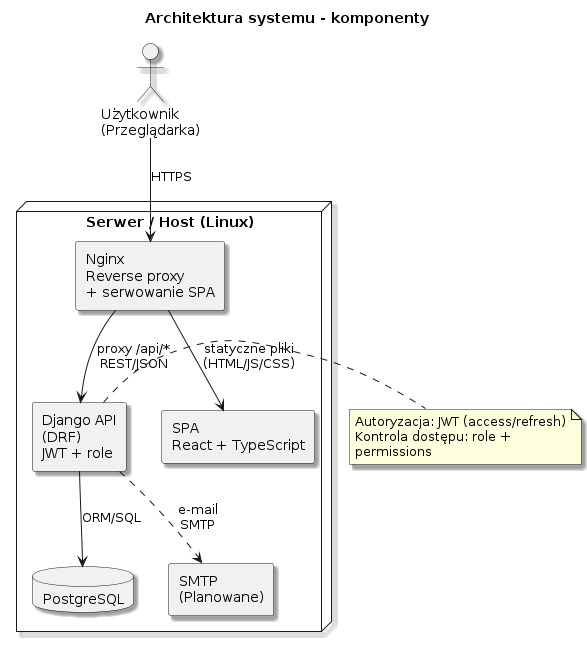
\includegraphics[width=0.7\linewidth]{resources/architektura_systemu.png}
\end{figure}

\subsection{Podział backendu na moduły}

Backend jest monolitem modularnym, podzielonym na trzy aplikacje domenowe:
\begin{itemize}
  \item \texttt{accounts} – konta użytkowników, role, logowanie i tokeny JWT,
  \item \texttt{school} – grupy i typy zajęć, sesje zajęć, zapisy, obecności,
  \item \texttt{billing} – produkty, należności miesięczne (\texttt{Purchase}), ręczne oznaczanie wpłat jako opłaconych.
\end{itemize}

Dodatkowe elementy:
\begin{itemize}
  \item SMTP – wysyłka e-mail (np. potwierdzenia/przypomnienia),
  \item zadania cykliczne – np. generacja rozliczeń i/lub przypomnienia.
\end{itemize}

\begin{figure}[H]
  \centering
  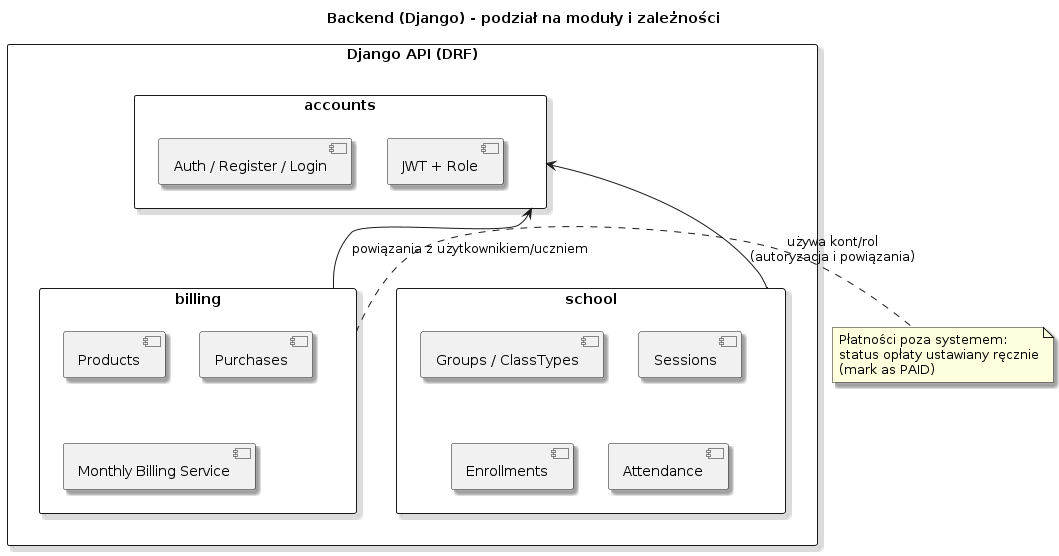
\includegraphics[width=0.9\linewidth]{resources/podzial_na_moduly.png}
\end{figure}

\subsection{Zastosowane szablony architektoniczne}

W projekcie zastosowano:
\begin{itemize}
  \item architekturę client--server (SPA jako klient, Django API jako serwer),
  \item komunikację REST/JSON pomiędzy SPA i backendem,
  \item monolit modularny po stronie backendu (moduły domenowe jako Django apps),
  \item podejście MVC/MVT: modele w ORM, logika w endpointach DRF (ViewSety/serwisy), prezentacja w SPA.
\end{itemize}

\subsection{Interfejsy kluczowych elementów oraz interakcje}

Komunikacja i interfejsy:
\begin{itemize}
  \item HTTPS: przeglądarka $\leftrightarrow$ Nginx,
  \item REST/JSON: SPA $\leftrightarrow$ backend (ścieżka \texttt{/api/*}),
  \item JWT: nagłówek \texttt{Authorization: Bearer <token>},
  \item SQL/ORM: backend $\leftrightarrow$ PostgreSQL,
  \item (plan) SMTP: backend $\leftrightarrow$ serwer pocztowy.
\end{itemize}

Najważniejsze scenariusze interakcji:
\begin{itemize}
  \item logowanie użytkownika i autoryzacja żądań przez JWT,
  \item generacja rozliczeń miesięcznych i ręczne oznaczenie wpłaty jako opłaconej.
\end{itemize}

\begin{figure}[H]
  \centering
  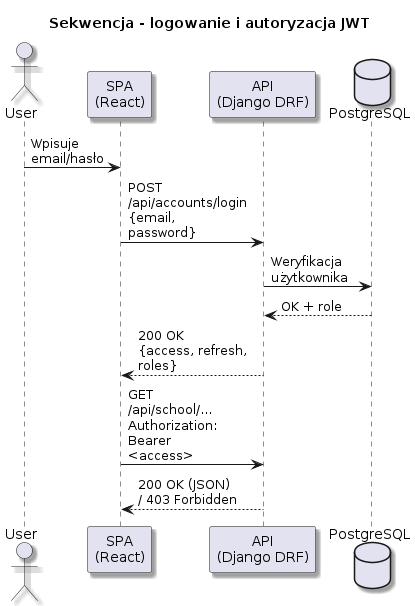
\includegraphics[width=0.7\linewidth]{resources/sekwencja_logowanie_autoryzacja.png}
\end{figure}

\begin{figure}[H]
  \centering
  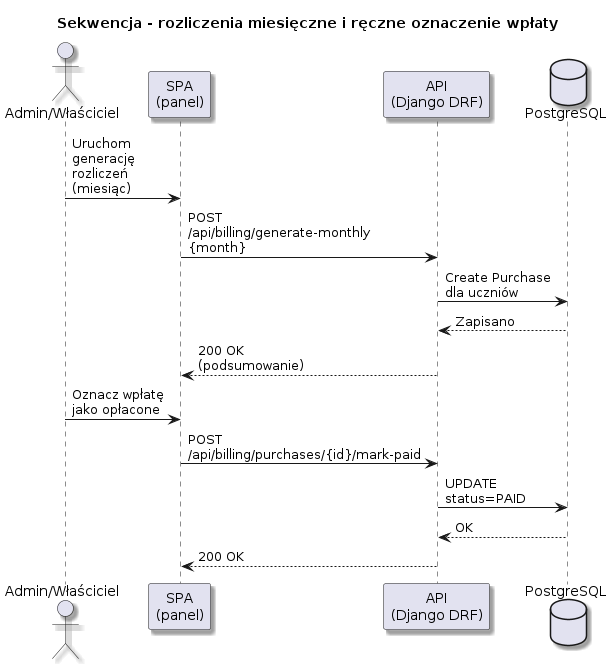
\includegraphics[width=0.7\linewidth]{resources/rozliczenia.png}
\end{figure}

\subsection{Perspektywa logiczna/funkcjonalna}

Zakres funkcjonalny systemu obejmuje:
\begin{itemize}
  \item konta użytkowników i role,
  \item planowanie oraz obsługę zajęć (sesje, zapisy, obecność),
  \item rozliczenia miesięczne oraz statusy opłat.
\end{itemize}

Warstwa UI znajduje się w SPA. Backend realizuje logikę biznesową, walidacje oraz kontrolę dostępu.

\subsection{Perspektywa sprzętowa (deployment) i środowisko uruchomieniowe}

Docelowe uruchomienie zakłada serwer z systemem Linux (np. Ubuntu/Debian) oraz konteneryzację (Docker Compose).
Wystawiony na zewnątrz jest wyłącznie Nginx, natomiast backend i baza danych działają w sieci prywatnej.

Elementy środowiska uruchomieniowego:
\begin{itemize}
  \item Nginx – reverse proxy oraz serwowanie plików SPA,
  \item Django API (WSGI, np. Gunicorn) – obsługa endpointów REST,
  \item PostgreSQL – baza danych uruchomiona wewnątrz sieci prywatnej.
\end{itemize}

\subsection{System bazy danych i mechanizmy utrwalania danych}

Utrwalanie danych realizowane jest w PostgreSQL (dane kont, zajęć, zapisów, obecności i rozliczeń).
Dostęp do danych realizuje ORM Django.

Operacje utrzymaniowe:
\begin{itemize}
  \item migracje schematu bazy (narzędzia Django),
  \item trwałe przechowywanie danych (wolumen DB),
  \item kopie zapasowe (zakres wdrożeniowy/operacyjny).
\end{itemize}

\subsection{Raportowanie oraz analityka/BI}

Raportowanie operacyjne opiera się na danych rozliczeniowych:
\begin{itemize}
  \item generacja miesięcznych należności (\texttt{Purchase}),
  \item podgląd statusów opłat (np. lista zaległości na dany miesiąc).
\end{itemize}

Analityka/BI może zostać rozszerzona przez:
\begin{itemize}
  \item eksport danych (np. CSV),
  \item dedykowane endpointy raportowe w panelu administracyjnym.
\end{itemize}

\subsection{Mechanizmy zarządzania}

Zarządzanie projektem i wdrożeniem obejmuje:
\begin{itemize}
  \item CI (lint/test/build),
  \item proces wdrożeniowy wraz z migracjami bazy,
  \item logowanie operacyjne (logi aplikacji i kontenerów).
\end{itemize}

\subsection{Mechanizmy bezpieczeństwa}

Bezpieczeństwo systemu zapewniają:
\begin{itemize}
  \item szyfrowanie komunikacji przez HTTPS (terminacja TLS na Nginx),
  \item autoryzacja przez JWT (access/refresh),
  \item kontrola dostępu oparta o role i uprawnienia (RBAC, permissions),
  \item walidacja danych wejściowych (serializery DRF) i ograniczenia modeli,
  \item izolacja komponentów: API i PostgreSQL w sieci prywatnej (brak bezpośredniej ekspozycji).
\end{itemize}

\begin{figure}[H]
  \centering
  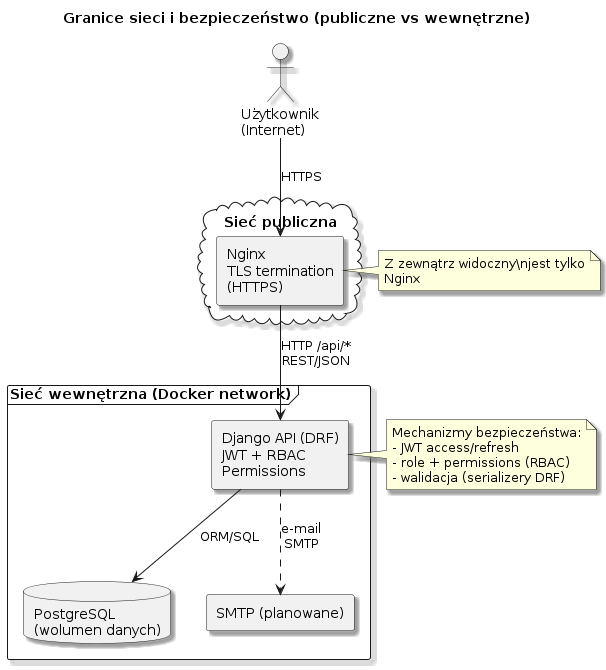
\includegraphics[width=0.7\linewidth]{resources/bezpieczenstwo.png}
\end{figure}

\section{Dane trwałe}
\subsection{Model logiczny danych}

Model danych został zaprojektowany w podejściu relacyjnym i obejmuje trzy główne obszary:
konta i role użytkowników, obsługę zajęć (grupy, sesje, zapisy, obecności) oraz rozliczenia.
Diagram ER przedstawia zależności pomiędzy encjami oraz kluczowe ograniczenia spójności (m.in. relacje
wiele-do-jednego oraz ograniczenia unikalności).

Ze względu na rozmiar diagramu, w treści pracy zamieszczono link, pod którym znajduje się pełna wersja diagramu.(zaleca się pobrać, bo przy podglądzie może być gorszej jakośći)

\href{https://drive.google.com/file/d/1GeEPdo2H1-CJX1YiavW60V5RUC897051/view?usp=sharing}{\textbf{Pobierz pełny diagram ER (PDF)}}

\subsection{Przetwarzanie i przechowywanie danych}

Dane systemu są przechowywane w relacyjnej bazie PostgreSQL. Dostęp do danych realizuje backend Django
z wykorzystaniem ORM, co zapewnia spójne mapowanie modeli domenowych na tabele oraz ułatwia utrzymanie schematu.

Operacje na danych są wykonywane poprzez REST API (Django REST Framework). Walidacja danych wejściowych odbywa się
na poziomie serializerów DRF oraz ograniczeń modeli, a kontrola dostępu do operacji jest realizowana przez JWT
(access/refresh) oraz uprawnienia zależne od ról użytkownika.

Zmiany schematu bazy danych są wprowadzane poprzez migracje Django, wersjonowane w repozytorium. W bazie stosowane
są indeksy i ograniczenia unikalności wspierające integralność danych (np. brak duplikatów zapisów na grupę
dla tego samego ucznia). Nie zakłada się programowania logiki biznesowej bezpośrednio w bazie danych (np. wyzwalaczy);
logika pozostaje po stronie backendu, co upraszcza rozwój i testowanie aplikacji.

\section{Specyfikacja testów}
Aplikację testowaliśmy zgodnie ze scenariuszami, które wyniknęły z~przypadków użycia.
Te testy były manualne i wykonywał je recenzent przed dopuszczeniem nowej
zmiany do gałęzi głównej repozytorium. Przed prezentacją aplikacji ponownie
upewniliśmy się, że wszystko działa.

\subsection{Standardy jakości}
Oprócz weryfikacji poprawności aplikacji w sensie logiki biznesowej powinnością
recenzenta było, pilnowanie zgodności aplikacji z pewnymi standardami. Potrzebę
spełnienia tych standardów narzucają wymagania \textbf{N1} i~\textbf{N3}.

\paragraph{Urządzenia mobilne} Interfejs powinien działać również na wąskich ekranach.
\paragraph{Dostępność} Interfejs nie powinien generować błędów związanych z~dostępnością,
    np. niski kontrast, niepodpisane przyciski.


\subsection{Testy jednostkowe}
Aby wcześnie wykrywać nowopowstałe błędy oraz przyspieszyć proces testowania,
oraz polepszyć strukturę kodu korzystaliśmy z testów jednostkowych.

Użyliśmy ich zarówno na frontendzie, jak i na backendzie. Na backendzie testowaliśmy
zachowanie endpointów. Przykładowo, poprawna prośba o zapisanie ucznia do grupy
zajęciowej powinna skutkować pozytywną odpowiedzią serwera oraz utworzeniem
odpowiednich wpisów w bazie danych.

\subsubsection{Sytuacje wyjątkowe}
Testy jednostkowe pozwalają również sprawdzić to, czego nie da się sprawdzić poprzez
interfejs. W szczególności reakcję serwera na zapytanie złośliwie spreparowane
z pominięciem interfejsu. Próba zarejestrowania do nieistniejącej grupy powinna
skutkować komunikatem o niepowodzeniu, a nie błędem serwera.

\subsubsection{Obsługa sytuacji wyjątkowych}
Gdy zostanie wykryta sytuacja wyjątkowa, np. dane ucznia nie zawierają daty urodzenia,
kod to wykrywa i zgłasza wyjątek. Serwer jest tak skonfigurowany, że ten błąd
przekształca na odpowiedź, która mówi, co jest źle w którym polu formularza.

Taki komunikat wyświetlamy na czerwono pod odpowiednim polem formularza.

\subsubsection{Automatyczne testy interfejsu}
Pisząc niektóre komponenty interfejsu, wspomogliśmy się testami jednostkowymi.
Przetestowaliśmy między innymi czy motyw kolorystyczny interfejsu zapisuje się
między sesjami oraz, czy przy pierwszej wizycie dostosowuje się do preferencji
zapisanych w przeglądarce.

\subsubsection{Miary jakości testów}
Nie korzystaliśmy z miary pokrycia kodu testami. Uznaliśmy, że biorąc pod uwagę
nasze niskie doświadczenie, mogłoby to doprowadzić do pisania testów „pod” pokrycie,
a nie takich, które są użyteczne.


\section{Wirtualizacja / konteneryzacja}
Użyliśmy kontenerów dockerowych, które symulują środowisko wdrożeniowe, przybliżając
je do programisty. Jednocześnie wymusza to, aby cała konfiguracja istotna z punktu
widzenia wdrożenia była zawarta w repozytorium. Niweluje to szansę wystąpienia
sytuacji, w~której to, że aplikacja działa, jest efektem jakiejś niejawnej
specyfiki/konfiguracji komputera programisty.

\section{Bezpieczeństwo}
Bezpieczeństwo danych oparte jest na identyfikatorach sesji, które są
tak zwanymi „secure cookies”. Serwer korzysta wyłącznie z połączeń szyfrowanych.
Z tych powodów, poufność identyfikatora jest odporna na ataki XSS
oraz man-in-the-middle. W praktyce pozostaje bezpieczeństwo hasła oraz
złośliwe oprogramowanie, które mogło zainfekować przeglądarkę, ale to
leży w gestii użytkownika.

\subsection{Uprawnienia użytkowników}
Każdy użytkownik ma przypisaną jedną z trzech ról: uczeń, instruktor albo admin.
Jest jeszcze superadmin, ale może się on zalogować tylko z sieci prywatnej między
kontenerami.

Role są przydzielane do kont, a konto jest związane z identyfikatorem sesji, który
otrzymuje użytkownik po zalogowaniu się, i który następnie służy do identyfikacji
użytkownika. Tak więc, złamanie ról wymaga podszycia się pod użytkownika z daną
rolą, co, jak wyjaśniliśmy powyżej, jest bardzo trudne, nie znając jego hasła.

Role są wykorzystywane do określenia czy dany użytkownik ma dostęp do danej operacji.
Np. tylko administrator może dodać grupę zajęciową, użytkownik ma dostęp jedynie
do odczytu.

\end{document}
